\documentclass[twocolumn, twocolappendix]{aastex631}
\received{\today}
\shorttitle{Giant Planet Formation}
\graphicspath{{figures/}}

\usepackage{lipsum}
\usepackage{physics}
\usepackage{multirow}
\usepackage{xspace}
\usepackage{natbib}
\usepackage{fontawesome5}
\usepackage{xcolor}
\usepackage{wrapfig}
\usepackage[figuresright]{rotating}

% remove indents in footnotes
\usepackage[hang,flushmargin]{footmisc} 

\newcommand{\todo}[1]{{\color{red}{[TODO: #1}]}}
\newcommand{\needcite}{{\color{magenta}{(needs citation)}}}
\newcommand{\placeholder}[1]{{\color{gray} \lipsum[#1]}}

% custom function for adding units
\makeatletter
\newcommand{\unit}[1]{%
    \,\mathrm{#1}\checknextarg}
\newcommand{\checknextarg}{\@ifnextchar\bgroup{\gobblenextarg}{}}
\newcommand{\gobblenextarg}[1]{\,\mathrm{#1}\@ifnextchar\bgroup{\gobblenextarg}{}}
\makeatother

\begin{document}

\title{{\huge Giant Planet Formation}\\\vspace{0.15cm}ASTR558 Final Project}

% affiliations
\newcommand{\UW}{Department of Astronomy, University of Washington, Seattle, WA, 98195}

\author[0000-0001-6147-5761]{T. Wagg}
\affiliation{\UW}

\correspondingauthor{Tom Wagg}
\email{tomjwagg@gmail.com}

\begin{abstract}
    \textbf{Background and Context:}
    \placeholder{1}
\end{abstract}

\keywords{}

\section{Key Concepts}

\begin{figure}
    \centering
    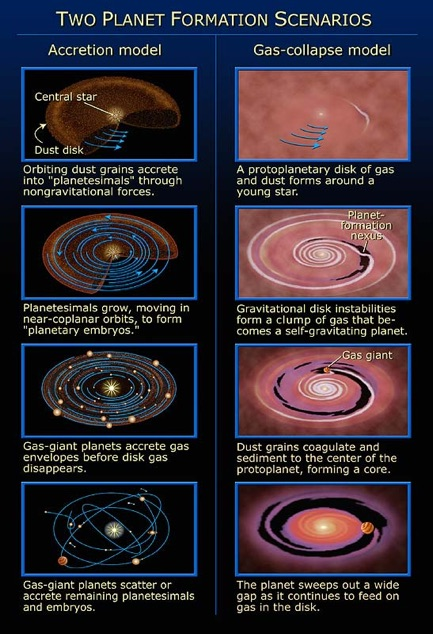
\includegraphics[width=\columnwidth]{channels_illustration.jpg}
    \caption{An illustration of different giant planet formation channels. (Credit: NASA and A. Feild (STScl))}
\end{figure}

\subsection{Core Accretion}

\citep{Pollack+1996}

\subsection{Direct Collapse}

\section{Recent Research}

\section{Quantitative Study}

\section{Unsolved Questions}

\bibliographystyle{aasjournal}
\bibliography{paper}{}

\end{document}